\documentclass{article}

\usepackage{../preamble}
\standalonetrue

\pagestyle{fancy}
\fancyhf{}
\rhead{Section \thesection}
\lhead{MATH 316 Lecture 15}
\rfoot{Page \thepage}


\title{MATH 316 Lecture 15}
\author{Ashtan Mistal}
\date{June 9, 2021}

\begin{document}

\ifstandalone
\maketitle
\fi

\graphicspath{{./Lecture15/}}

Last time, we learned about the solution for Laplace's equation. We did a few examples for Laplace's equation, and for these examples we got Dirichlet boundary conditions. Today, we'll do a few more examples for Laplace's equation including Neumann boundary conditions. 

\section{Examples}

\subsection{Example 15: Neumann Boundary Condition for Laplace Equation}

Domain is from $0 < x < a$, and from $0 < y < b$:

\begin{center}
    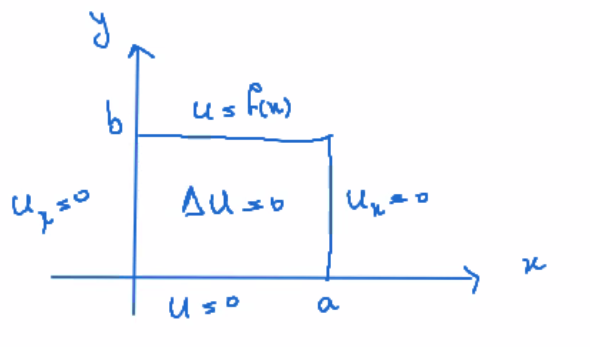
\includegraphics[width = 0.6 \textwidth]{1.png}
\end{center}

Here, we have one inhomogeneous boundary condition.North BVP: $u(x,t) = X(x) Y(y)$. Substitute into Laplacian in order to get $\frac{X''}{X} = - \frac{Y''}{Y} = - \lambda$ where $\lambda$ is a constant. We choose the sign of $\lambda$ such that $\frac{X''}{X}$ becomes similar to a P2 boundary condition. Let's write the boundary condition: 

$X(x)$ problem: $x'(0) = 0, \quad X'(a) = 0$. The PDE is therefore a P2 problem, with $X'' + \lambda X = 0$. Hence, we have eigenvalues of $\lambda_n = \left( \frac{n \pi}{a} \right)^2$ for $n \in \NN$, and an eigenfunction of $X_n (x) = \cos \left( \frac{n \pi x}{a} \right)$. As $\lambda_0 \to 0, X_0(x) = 1$. 

$Y(y)$ problem: We have $Y_n'' - \left( \frac{n \pi}{a} \right)^2 Y_n = 0$ and $Y(0) = 0$. For $n = 0$, the first term vanishes and we get a solution of $Y_0(y) = Ay + B$. Given boundary conditions this becomes $Y_0(y) = A y$. For $n \geq 1$, $Y_n (y) = \sinh \left( \frac{n \pi}{a} y \right)$ using similar steps as previous lectures. 

Therefore, $u(x,y) = C_0 y + \sum_{n=1}^\infty C_n \cos \left(\frac{ n \pi x}{a} \right) \sinh \left( \frac{n \pi}{a} y \right)$

$$f(x) = u(x,b) = C_0 b + \sum_{n=1}^\infty C_n \left( \frac{n \pi}{a} b \right) \cos \left( \frac{n \pi x}{a} \right)$$

We therefore need a Fourier cosine series for $f(x)$: $f(x) = \frac{a_0}{2} + \sum_{n=1}^\infty a_n \cos \left( \frac{n \pi x}{a} \right)$

If we match up the coefficients, we get:

$$\Rightarrow C_0 b = \frac{a_0}{2} \Rightarrow C_0 = \frac{a_0}{2b}$$

and $C_n \sinh \left( \frac{n \pi}{a} b \right) = a_n \Rightarrow C_n = \frac{a_n}{\sinh \left( \frac{n \pi}{a} b \right)}$

Therefore we get the following solution:

$$\Rightarrow u(x,y) = \frac{a_0}{2b} y + \sum_{n=1}^\infty a_n \cos \left( \frac{n \pi x}{a} \right) \frac{ \sinh \left( \frac{n \pi}{a} y \right)}{\sinh \left( \frac{n \pi}{a} b \right)}$$

\subsection{Example 16: Neumann boundary conditions on 4 sides}

Let's first sketch the problem:

here, we're given $a = 2$ and $b = 1$. 

\begin{center}
    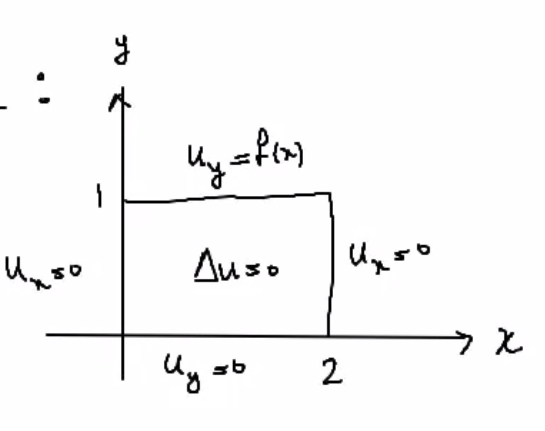
\includegraphics[width = 0.6 \textwidth]{3.png}
\end{center}

where: a) $f(x) = x-1$, and b) $f(x) = x+1$. \footnote{What goes wrong in b) and why?}

Let's start with the $X(x)$ problem. Here, we separate variables as before. So, we get the following:

$$\lambda_0 = 0 \to X_0(x) = 1$$

$$\lambda_n = \left( \frac{n \pi}{2} \right)^2 \to X_n (x) = \cos ( \frac{n \pi x}{2} ) \text{ for } n \in \NN$$

$Y(y)$ problem:

$Y_n'' = \lambda_n Y_n$ and $Y_n '(0) = 0$. For $n = 0$, we get $Y_0 = 1$ and for $n \geq 1$ we get $Y_n (y) = C_1 e^{\frac{n \pi}{2} y } + C_2 e^{ - \frac{n \pi y}{2}}$. 

We take the derivative of this to make it look like $\sinh$ or $\cosh$. 

$$Y_n'(y) = \frac{n \pi}{2} \left( C_1 e^{ \frac{n \pi y}{2}} - C_2 e^{- \frac{n \pi y}{2}} \right)$$

At $y = 0$:

$$Y_n'(0) = C_1 - C_2 = 0 \Rightarrow C_1 = C_2$$

Therefore, we get the following solution:

$$Y_n' = \cosh \left( \frac{n \pi y}{2} \right)$$

Now let's find a series solution:

$$u(x,y) = C_0 + \sum_{n=1}^\infty C_n \cos \left( \frac{n \pi x}{2} \right) \cosh \left( \frac{n \pi y}{2} \right)$$

Now let's substitute the other boundary conditions, now that we have the general solution:

At $y = 1$, $u_y = f(x)$. Therefore, we need to find the Fourier cosine series for $f(x)$: (Take the derivative of the previous series)

$$u_y (x,y) = \sum_{n=1}^\infty C_n \left( \frac{n \pi}{2} \right) \cos \left( \frac{n \pi x}{2} \right) \sinh \left( \frac{n \pi y}{2} \right)$$

Part a): $f(x) = x-1$. 

The Fourier cosine series for $f(x)$ is through the following:

$$a_0 = \frac{2}{2} \int_0^2 (x-1) dx = 0$$

$$a_n = \frac{2}{2} \int_0^2 (x-1) \cos \left( \frac{n \pi}{2} x \right) dx = \underbrace{\left. \frac{2}{n\pi} (x-1) \sin \left( \frac{n \pi x}{2} \right) \right|_0^2}_{ = 0} - \frac{2}{n \pi} \int_0^2 \sin \left( \frac{n \pi x}{2} \right) dx$$

%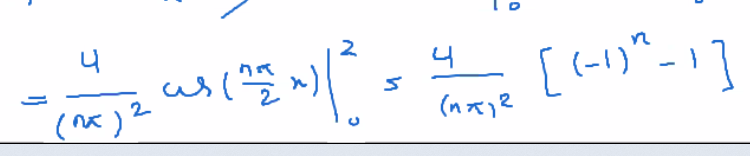
\includegraphics[width = 0.5 \textwidth]{4.png}

$$\Rightarrow a_n = \left. \frac{4}{(n \pi)^2} \cos \left( \frac{n \pi x}{2} \right) \right|_0^2 = \frac{4}{(n \pi)^2} [(-1)^n - 1]$$

$$\Rightarrow C_n = \frac{8}{(n \pi)^3} \frac{ [(-1)^2 - 1]}{\sinh \left( \frac{n \pi}{2} \right)} \text{ for } n \in \NN$$

Therefore,

$$u(x,y) = C_0 + \sum_{n=1}^\infty \frac{8}{(n \pi)^3} \frac{ [(-1)^2 - 1]}{\sinh \left( \frac{n \pi}{2} \right)}  \cos \left( \frac{n \pi x}{2} \right) \cosh \left( \frac{n \pi y}{2} \right)$$

where $C_0$ is an arbitrary constant. 

\textbf{What about part b?}

We have $f(x) = x+1$. If we calculate $a_0$, it becomes $a_0 = \frac{2}{2} \int_0^2 (x_1) dx = \left. \left( \frac{x^2}{2} + x \right) \right|_0^2 = 4$. 

For $a_n$, we have:

$$a_n = \frac{2}{2} \int_0^2 (x+1) \cos \left( \frac{n \pi x}{2} \right) dx = \frac{2}{n \pi} (x+1) \left. \sin \left( \frac{n \pi x}{2} \right) \right|_0^2 - \frac{2}{n \pi} \int_0^2 \sin \left( \frac{n \pi x}{2} \right) dx$$

$$a_n = \frac{4}{(n \pi)^2} \left[ (-1)^n - 1 \right]$$

Let's match the coefficients:

$$C_n = \frac{8}{(n \pi)^3} \frac{ \left[ (-1)^n - 1 \right] }{\sinh \frac{n \pi}{2}}, \quad \text{ for } n \in \NN$$

But here, we have an $a_0$ that doesn't appear in the form of $u_y$. There's nothing to match it to. There is an issue with the convergence. Because we cannot match the $a_0$ term, there is no solution by this method. 

What's the difference between a) and b)?

$$\int_0^2 f(x) dx = \left\{ \begin{matrix} 0 & (a) \\ 4 & (b) \end{matrix} \right.$$

\begin{center}
    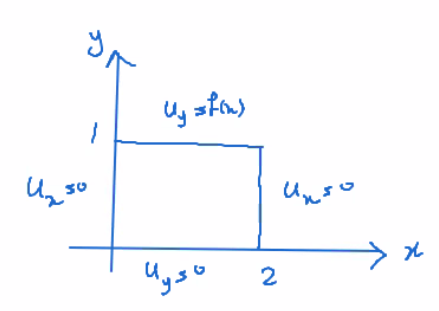
\includegraphics[width = 0.6 \textwidth]{5.png}
\end{center}

The condition on East, South, and West physically means that there is no heat flow (isolated). 

On N (north): a) $\int_0^2 f(x) dx = 0$. The average heat flux is equal to zero. 

\hfill

b) $\int_0^2 f(x) dx = 4 \neq 0$. Here, it says that heat is entering domain through the north wall, but not leaving through East, South, or West. As a result, there is \textbf{no steady state}. 

Earlier, we talked about the arbitrary constant $C_0$. In part A, $C_0$ is the average "initial" temperature. 

\subsection{Example 17: Both Boundary Conditions}

$\Delta u = 0$, with $u_x(0,y) = 0$ and $u_x (a,y) = g(x)$, with $u(x,0) = f(x)$ and $u(x,b) = 0$. $y \in [0,b]$ and $x \in [0,a]$

$$u(x,y) = u_S(x,y) + u_E (x,y)$$
\begin{center}
    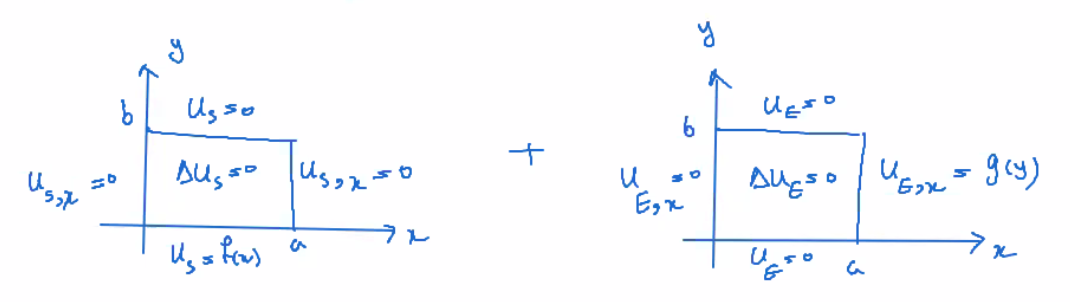
\includegraphics[width = 0.7 \textwidth]{6.png}
\end{center}

On South:

(We know it's going to be FCS because of boundary conditions)

$$u_S (x,y) = C_0 + \sum_{n=1}^\infty C_n \cos \left( \frac{n \pi x}{a} \right) \sinh \left( \frac{n \pi}{a} (y-b) \right)$$

$$f(x) = \frac{a_0}{2} + \sum_{n=1}^\infty a_n \cos \left( \frac{n \pi x}{a} \right)$$

(Boundary condition on south wall, $u(x,0) = f(x)$

We then need to evaluate $C_0$ and $C_n$:

$$C_0 = \frac{a_0}{2}$$

$$C_n = \frac{- a_n}{\sinh \left( \frac{n \pi b}{a} \right)}$$

Substitute into $u_S(x,y)$ gives us the solution. 

On East (Exercise):
$$u_E(x,y) = \sum_{n=1}^\infty d_n \sin \left( \frac{n \pi y}{b} \right) \cosh \left( \frac{n \pi x}{b} \right)$$

$$\left. \frac{\partial u_E}{\partial x} \right|_{x=a} = \left. \sum_{n=1}^\infty d_n \left( \frac{n \pi}{b} \right) \sinh \left( \frac{n \pi x}{b} \right) \sin \left( \frac{n \pi y}{b} \right) \right|_{x=a} = g(y)$$

FSS for $g(y)$:

$$g(y) = \sum_{n=1}^\infty b_n \sin \left( \frac{n \pi y}{b} \right)$$

From the previous two equation, we get the following:

$$d_n = \frac{ b_n \cdot b}{n \pi \sinh \left( \frac{n \pi a}{b} \right) }$$


%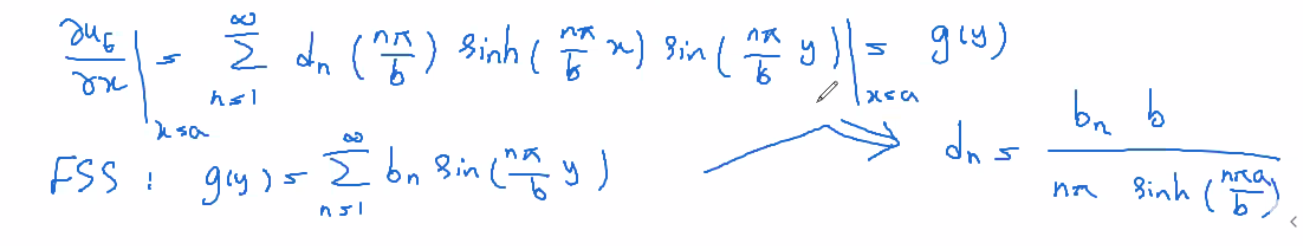
\includegraphics[width = 0.7 \textwidth]{9.png}


And therefore

$$u_E (x,y) = \sum_{n=1}^\infty \frac{b \cdot b_n}{n \pi \sinh ( \frac{n \pi a}{b} )} \sin \left( \frac{n \pi y}{b} \right) \cosh \left( \frac{n \pi x}{b} \right)$$

Finally, we have $u(x,y) = u_S (x,y) + u_E(x,y)$

\subsection{Example 18: Laplace equations in Circular Domain}

$$\Delta u = u_{rr} + \frac{1}{r} u_r + \frac{1}{r^2} u_{\theta \theta} = 0$$

with $(r, \theta) \in \Omega$

$u(a,\theta = f(\theta)$, with $\theta \in [0, 2 \pi]$. $u(r, \theta)$ is bounded as $r \to 0$

Separation of variables: $u(r, \theta) = R(r) \Theta (\theta) \to u_r = R' (\theta)$, and $u_{\theta} = R \Theta '$. $u_{rr} = R'' \Theta$, and $u_{\theta \theta} = R \Theta''$

Substitute:

$$R'' \Theta + \frac{1}{r} R' \Theta + \frac{1}{r^2} R \Theta'' = 0$$

Simplifying:

$$\frac{\Theta ''}{\Theta} = - \left( \frac{r^2 R''}{R} + \frac{r R'}{R} \right) = - \lambda$$

Starting with $\Theta$:
$$\Theta'' + \lambda \Theta = 0$$

$$\Theta(0) = \Theta (2 \pi)$$

$$\Theta'(0) = \Theta'( 2 \pi)$$

i.e. $\Theta (\theta)$ is a periodic, P3, boundary value problem. 

hence we have the following eigenvalues:

$$\lambda_n = \left( \frac{n \pi}{\pi} \right)^2 = n^2 \text{ for } n \in \NN$$

Eigenfunction:

%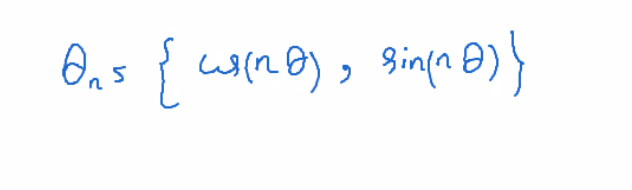
\includegraphics[width = 0.5 \textwidth]{10.png}

$$\Theta_n = \left\{ \cos(n \theta), \sin(n \theta) \right\}$$

We will finish this example in class tomorrow. 




\end{document}